\documentclass[a4paper, british]{article}

\usepackage[utf8]{inputenc}
\usepackage[T1]{fontenc}
\usepackage{babel}
% \usepackage[margin=2.5cm,a4paper]{geometry}
% \usepackage[skip=1em]{parskip}
\usepackage{lmodern} 
\usepackage{microtype}
% \usepackage{xcolor}
\usepackage{graphicx}
\graphicspath{ {./figures/} }
% \usepackage{float}
% \usepackage{enumitem}
\usepackage{adjustbox} % rescale - useful for Dia exported TeX
\usepackage{tikz}
% \usepackage{pgfplots}
\usepackage{booktabs} %tables no vertical lines
\usepackage{enumitem}
% \usepackage{array}
% \usepackage{authblk}
% \usepackage{fancyhdr} %headers and footers
% \usepackage{titlesec}
% \usepackage{tcolorbox} % framed text boxes
% \usepackage{mathtools, amssymb, amsthm}
% \usepackage{gensymb}
%\usepackage{pygmentize}
\usepackage{minted} % code highlighting
\usepackage{chemformula} % chemical formulae
\usepackage{chemfig} % molecular figures
\usepackage{siunitx}
\usepackage{csquotes}
\usepackage[titletoc, title]{appendix}
% \usepackage{lettrine} % initials

\usepackage[
pdfauthor={Adam Menne},
pdftitle={Applied Mathematics - Assignment 2},
pdfsubject={},
pdfkeywords={}]{hyperref}

\usepackage[noabbrev]{cleveref}

\usepackage[
backend=biber,
style=numeric,
sorting=none,
doi=true,
isbn=false
]{biblatex}
\addbibresource{citations.bib}

\setlength{\parskip}{1em}
\setlength{\parindent}{0em}
\linespread{1.3}

\title{Applied Mathematics - Assignment 2}
\date{Last editted on \today}
\author{Adam Menne - 24942901\\ Stellenbosch University}

\begin{document}

\maketitle

\vspace{40mm}

\tableofcontents

\newpage

\section{Problem 1}

\subsection*{(a), (b), (c)}

\begin{figure}[H]
    \centering
    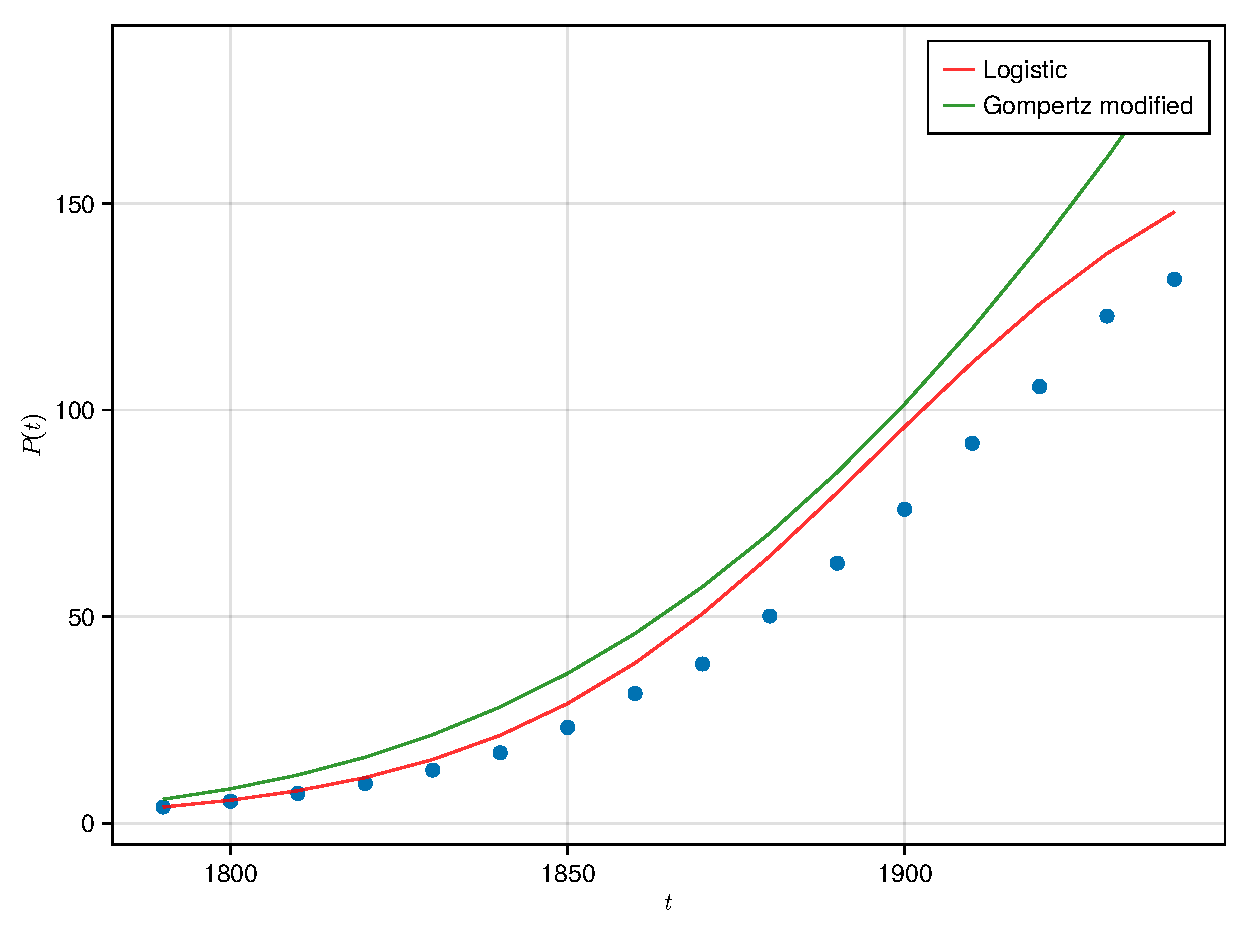
\includegraphics[width=\textwidth]{figures/fig1.pdf}
    \caption{}
    \label{fig:1}
\end{figure}

\begin{figure}[H]
    \centering
    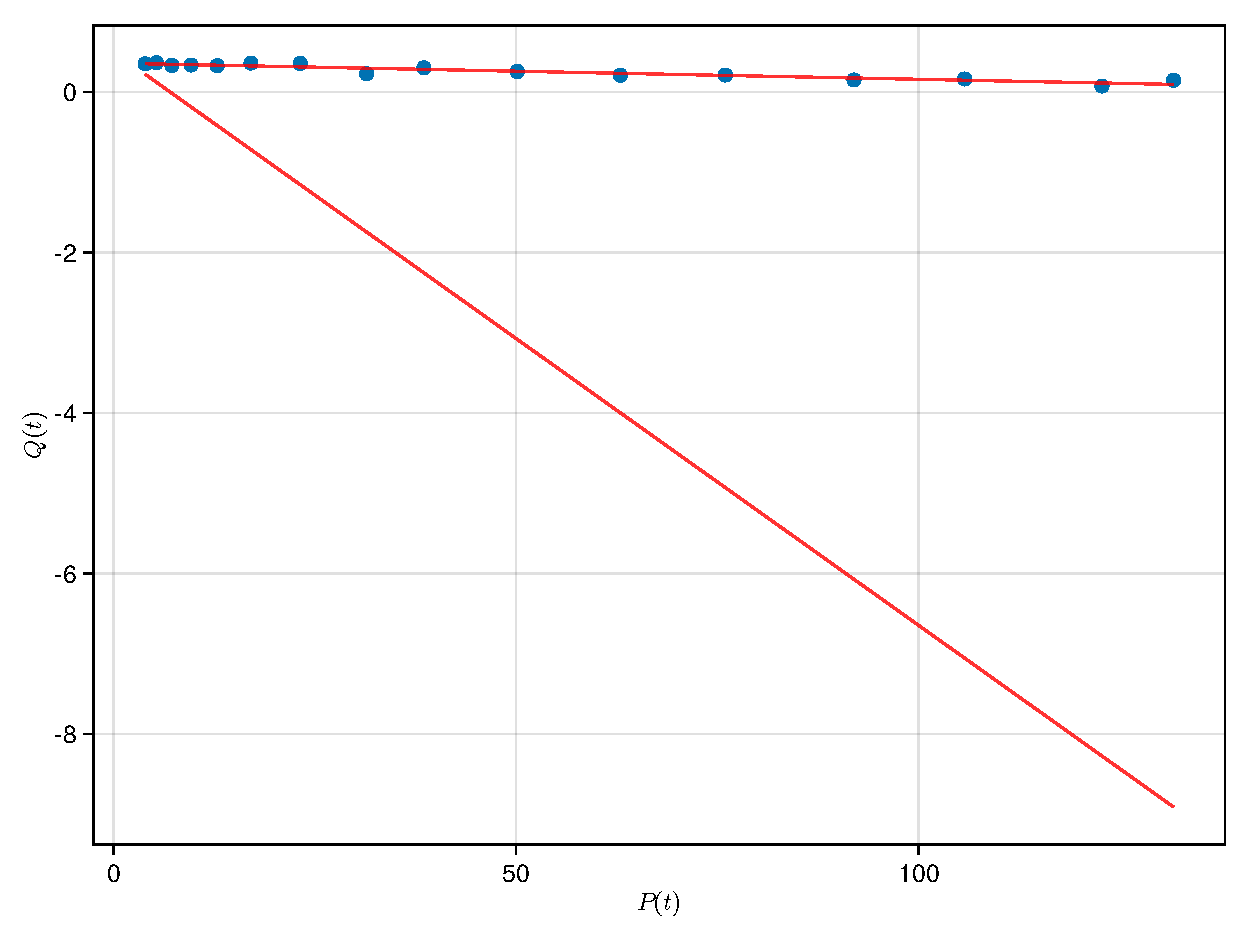
\includegraphics[width=\textwidth]{figures/fig2.pdf}
    \caption{}
    \label{fig:2}
\end{figure}

\subsection*{(d)}

176.2 million with \(K =\) 178.1 million. In 2020 the actual US population was 329.5

\section{Problem 2}

\subsection*{(a)}

\subsubsection*{Solving the differential equation}

\[\frac{dP}{dt} = P(a-b\ln P)\]

\[\int \frac{1}{P(a-b\ln P)}\ dP = \int dt\]

\[u = \ln P \quad ,\ du = \frac{1}{p}\ dP\]

\[\int \frac{1}{a-bu}\ du = t + c\]

\[s = a-bu \quad ,\ ds = -b\ du\]

\[-\frac{1}{b}\ \int \frac{1}{s}\ ds = t+c\]

\[- \frac{\ln (s)}{b} = t+c\]

\[- \frac{\ln (a-bu)}{b} = t + c\]

\[- \frac{\ln (a-b \ln (P))}{b} = t + c\]

\[\ln (a-b \ln (P)) = -bt + c\]

\[a-b \ln (P) = ce^{-bt}\]

\[\ln P = \frac{ce^{-bt}-a}{-b}\]

\[P = e^{\frac{a}{b} + ce^{-bt}}\]

\subsubsection*{Solving the IVP}

\[P_0 = e^{\frac{a}{b}} e^{ce^{-b(0)}}\]

\[P_0 = e^{\frac{a}{b}+c}\]

\[\ln P_0 = \frac{a}{b} + c\]

\[c = \ln P - \frac{a}{b}\]

\subsection*{(b)}

% \begin{minted}{julia}
%     p2 = Polynomials.fit(log.(pop[1:16]), Q1.(1:16), 1)
%     a2, b2 = p2.coeffs[1], -p2.coeffs[2]
% \end{minted}

See \cref{fig:1}

\subsection*{(c)}

See \cref{fig:2}

\subsection*{(e)}

2089.5

 Full source code for this assignment is availble at \url{https://github.com/AdamMenne/applied_mathematics_244/tree/master/assignment_2}

\end{document}